% !TeX root = ../libro.tex
% !TeX encoding = utf8
%
%*******************************************************
% Introducción
%*******************************************************

% \manualmark
% \markboth{\textsc{Introducción}}{\textsc{Introducción}} 
\chapter{Resumen}

%De acuerdo con la comisión de grado, el TFG debe incluir una introducción en la que se describan claramente los objetivos previstos inicialmente en la propuesta de TFG, indicando si han sido o no alcanzados, los antecedentes importantes para el desarrollo, los resultados obtenidos, en su caso y las principales fuentes consultadas.

%En este capítulo, resumiremos el proceso que hemos seguido hasta llegar a la demostración, desde una perspectiva algorítmica, del Primer Teorema de Incompletitud. En la \cref{fig:resumen}, se puede observar un esquema resumen de este trabajo, el cual es extendido en la \cref{fig:resumen-extendido}. En este resumen final se omiten las \cref{part:introduccion,,part:conclusion}.

Comenzamos este Trabajo de Fin de Grado con el \cref{ch:motivacion}, que destaca la motivación que subyace este trabajo, así como los objetivos que se pretenden cumplir. Inmediatamente después, en el \cref{ch:historia}, hacemos una breve contextualización histórica de esta obra.

El desarrollo teórico comienza con el \cref{ch:programas-python-maquinas-turing}, en cuya \cref{sec:programas-python} introducimos una clase específica de programas en Python, los \emph{programas SISO}, y observamos que esta clase es tan expresiva como la clase de todos los programas en Python. A continuación, en la \cref{sec:maquinas-turing}, profundizamos en las \emph{máquinas de Turing}, herramienta matemática principal de nuestro trabajo. En la \cref{sec:equivalencia}, introducimos nuevos modelos de computación equivalentes, hasta llegar al resultado principal del capítulo: que las máquinas de Turing pueden simular programas en Python, y viceversa; en otras palabras, que los programas en Python y las máquinas de Turing son equivalentes. Esto nos permitirá usar programas en Python convenientemente, sin realizar descripciones de máquinas de Turing. Concluimos introduciendo la tesis de Church-Turing en la \cref{sec:church-turing}, y viendo que la equivalencia probada puede ser un argumento a su favor.

En la \cref{sec:problemas-decidibles} definimos los \emph{problemas computacionales}, y observamos que los programas en Python (y, equivalentemente, las máquinas de Turing), pueden resolverlos. Llamamos \emph{decidibles} a aquellos problemas que pueden resolverse mediante un programa que nunca para. En la \cref{sec:universalidad} observamos que un programa puede simularse a sí mismo, lo cual nos conduce en la \cref{sec:problemas-no-decidibles} a la existencia de problemas no decidibles. En la \cref{sec:problemas-semidecidibles} relajamos la condición de parada para obtener problemas \emph{semidecidibles}. A continuación, introducimos en la \cref{sec:reducciones} la técnica de \emph{reducción}, que nos permite obtener nuevos problemas no decidibles, incluyendo el más importante del trabajo en la \cref{sec:problema-parada}: el \emph{problema de la parada}.

Para demostrar el teorema principal de este trabajo, es necesario formalizar los conceptos de \emph{demostración} y \emph{verdad}. Hacemos esto introduciendo los \emph{sistemas formales} en la \cref{sec:sistemas-formales} y los \emph{sistemas lógicos} en la \cref{sec:sistemas-logicos}. Los sistemas formales son \emph{sintácticos}: formalizan qué es un \emph{teorema}, una \emph{fórmula} demostrable a partir de un conjunto de \emph{axiomas} y \emph{reglas de inferencia}. Por otro lado, los sistemas lógicos incorporan a los sistemas formales un componente semántico: la \emph{verdad}. En las \cref{sec:solidez-completitud-decidibilidad,,sec:consistencia} presentamos propiedades esenciales de los sistemas mencionados, que relacionan los conceptos semánticos y sintácticos. Destacamos en la \cref{sec:aritmetica-peano} la introducción de la \emph{aritmética de Peano}: un sistema lógico de especial importancia.

Como culmen, en el \cref{ch:teorema-incompletitud} demostramos el Primer Teorema de Incompletitud: primero desde la aritmética de Peano en la \cref{sec:primera-aproximacion}, para luego generalizarlo mediante dos versiones. La primera, semántica, es demostrada en la \cref{sec:version-semantica}, y nos permite (bajo unas hipótesis computacionales) encontrar afirmaciones ciertas e indemostrables en sistemas lógicos. A continuación, la versión sintáctica de la \cref{sec:version-sintactica}, más cercana a la de Gödel, nos conduce a la existencia de sentencias indemostrables en sistemas formales. Finalizamos con la \cref{sec:consecuencias}, estudiando importantes consecuencias matemáticas (\cref{subsec:segundo-problema-hilbert}) y filosóficas (\cref{subsec:mente-humana-tesis-church-turing}).

Finalmente, terminamos con algunas conclusiones en el \cref{ch:conclusiones}, y dedicando unas palabras finales para el trabajo posterior en el \cref{ch:trabajo-futuro}.


%\vfill
% ====================
%\begin{figure}[H]
%\centering
%\vspace{8pt}
%\hspace*{-1cm}
%\centerline{
\tikzset{every picture/.style={line width=0.75pt}} %set default line width to 0.75pt        

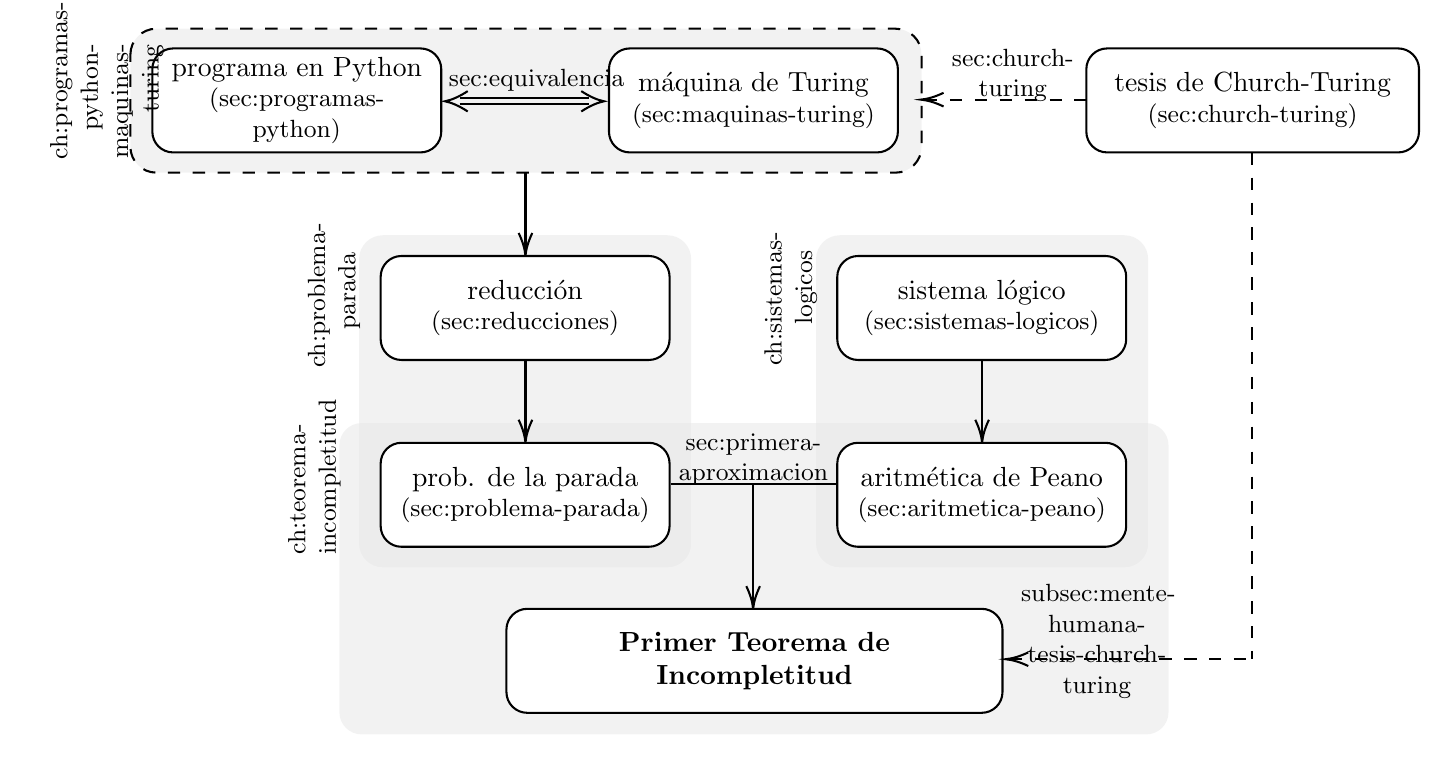
\begin{tikzpicture}[x=0.75pt,y=0.75pt,yscale=-1,xscale=1]
%uncomment if require: \path (0,446); %set diagram left start at 0, and has height of 446

%Rounded Rect [id:dp30270366230366363] 
\draw  [draw opacity=0][fill={rgb, 255:red, 230; green, 230; blue, 230 }  ,fill opacity=0.5 ] (130.5,359.59) .. controls (130.5,365.5) and (135.3,370.3) .. (141.21,370.3) -- (519.29,370.3) .. controls (525.2,370.3) and (530,365.5) .. (530,359.59) -- (530,231.02) .. controls (530,225.1) and (525.2,220.3) .. (519.29,220.3) -- (141.21,220.3) .. controls (135.3,220.3) and (130.5,225.1) .. (130.5,231.02) -- cycle ;
%Rounded Rect [id:dp4823897095202676] 
\draw  [draw opacity=0][fill={rgb, 255:red, 230; green, 230; blue, 230 }  ,fill opacity=0.5 ] (360.17,278.37) .. controls (360.17,284.69) and (365.28,289.8) .. (371.6,289.8) -- (508.74,289.8) .. controls (515.05,289.8) and (520.17,284.69) .. (520.17,278.37) -- (520.17,141.23) .. controls (520.17,134.92) and (515.05,129.8) .. (508.74,129.8) -- (371.6,129.8) .. controls (365.28,129.8) and (360.17,134.92) .. (360.17,141.23) -- cycle ;
%Rounded Rect [id:dp03353774001964016] 
\draw  [draw opacity=0][fill={rgb, 255:red, 230; green, 230; blue, 230 }  ,fill opacity=0.5 ] (140,278.37) .. controls (140,284.68) and (145.12,289.8) .. (151.43,289.8) -- (288.57,289.8) .. controls (294.88,289.8) and (300,284.68) .. (300,278.37) -- (300,141.23) .. controls (300,134.92) and (294.88,129.8) .. (288.57,129.8) -- (151.43,129.8) .. controls (145.12,129.8) and (140,134.92) .. (140,141.23) -- cycle ;
%Rounded Rect [id:dp33336382156813316] 
\draw  [fill={rgb, 255:red, 230; green, 230; blue, 230 }  ,fill opacity=0.5 ][dash pattern={on 4.5pt off 4.5pt}] (29.83,42.77) .. controls (29.83,35.88) and (35.41,30.3) .. (42.3,30.3) -- (398.54,30.3) .. controls (405.42,30.3) and (411,35.88) .. (411,42.77) -- (411,87.17) .. controls (411,94.05) and (405.42,99.64) .. (398.54,99.64) -- (42.3,99.64) .. controls (35.41,99.64) and (29.83,94.05) .. (29.83,87.17) -- cycle ;
%Rounded Rect [id:dp2990019894214928] 
\draw  [fill={rgb, 255:red, 255; green, 255; blue, 255 }  ,fill opacity=1 ] (40.4,49.82) .. controls (40.4,44.29) and (44.89,39.8) .. (50.42,39.8) -- (169.58,39.8) .. controls (175.11,39.8) and (179.6,44.29) .. (179.6,49.82) -- (179.6,79.88) .. controls (179.6,85.41) and (175.11,89.9) .. (169.58,89.9) -- (50.42,89.9) .. controls (44.89,89.9) and (40.4,85.41) .. (40.4,79.88) -- cycle ;
%Straight Lines [id:da7571263167258138] 
\draw    (188.42,63.77) -- (250.99,63.77)(188.42,66.77) -- (250.99,66.77) ;
\draw [shift={(257.99,65.27)}, rotate = 180] [color={rgb, 255:red, 0; green, 0; blue, 0 }  ][line width=0.75]    (10.93,-4.9) .. controls (6.95,-2.3) and (3.31,-0.67) .. (0,0) .. controls (3.31,0.67) and (6.95,2.3) .. (10.93,4.9)   ;
\draw [shift={(181.42,65.27)}, rotate = 0] [color={rgb, 255:red, 0; green, 0; blue, 0 }  ][line width=0.75]    (10.93,-4.9) .. controls (6.95,-2.3) and (3.31,-0.67) .. (0,0) .. controls (3.31,0.67) and (6.95,2.3) .. (10.93,4.9)   ;
%Straight Lines [id:da6359609928939494] 
\draw    (220.17,99.97) -- (220.17,137.64) ;
\draw [shift={(220.17,139.64)}, rotate = 270] [color={rgb, 255:red, 0; green, 0; blue, 0 }  ][line width=0.75]    (10.93,-3.29) .. controls (6.95,-1.4) and (3.31,-0.3) .. (0,0) .. controls (3.31,0.3) and (6.95,1.4) .. (10.93,3.29)   ;
%Straight Lines [id:da27008321467916896] 
\draw    (220.17,189.97) -- (220.17,227.64) ;
\draw [shift={(220.17,229.64)}, rotate = 270] [color={rgb, 255:red, 0; green, 0; blue, 0 }  ][line width=0.75]    (10.93,-3.29) .. controls (6.95,-1.4) and (3.31,-0.3) .. (0,0) .. controls (3.31,0.3) and (6.95,1.4) .. (10.93,3.29)   ;
%Straight Lines [id:da46114586121240286] 
\draw    (440.17,189.97) -- (440.17,227.64) ;
\draw [shift={(440.17,229.64)}, rotate = 270] [color={rgb, 255:red, 0; green, 0; blue, 0 }  ][line width=0.75]    (10.93,-3.29) .. controls (6.95,-1.4) and (3.31,-0.3) .. (0,0) .. controls (3.31,0.3) and (6.95,1.4) .. (10.93,3.29)   ;
%Straight Lines [id:da7285174494946591] 
\draw    (290.17,249.8) -- (370,249.8) ;
%Straight Lines [id:da15936204740305504] 
\draw    (329.86,249.97) -- (329.86,307.8) ;
\draw [shift={(329.86,309.8)}, rotate = 270] [color={rgb, 255:red, 0; green, 0; blue, 0 }  ][line width=0.75]    (10.93,-3.29) .. controls (6.95,-1.4) and (3.31,-0.3) .. (0,0) .. controls (3.31,0.3) and (6.95,1.4) .. (10.93,3.29)   ;
%Rounded Rect [id:dp7161475946545517] 
\draw  [fill={rgb, 255:red, 255; green, 255; blue, 255 }  ,fill opacity=1 ] (260.4,49.82) .. controls (260.4,44.29) and (264.89,39.8) .. (270.42,39.8) -- (389.58,39.8) .. controls (395.11,39.8) and (399.6,44.29) .. (399.6,49.82) -- (399.6,79.88) .. controls (399.6,85.41) and (395.11,89.9) .. (389.58,89.9) -- (270.42,89.9) .. controls (264.89,89.9) and (260.4,85.41) .. (260.4,79.88) -- cycle ;
%Rounded Rect [id:dp7743968693248953] 
\draw  [fill={rgb, 255:red, 255; green, 255; blue, 255 }  ,fill opacity=1 ] (150.4,149.82) .. controls (150.4,144.29) and (154.89,139.8) .. (160.42,139.8) -- (279.58,139.8) .. controls (285.11,139.8) and (289.6,144.29) .. (289.6,149.82) -- (289.6,179.88) .. controls (289.6,185.41) and (285.11,189.9) .. (279.58,189.9) -- (160.42,189.9) .. controls (154.89,189.9) and (150.4,185.41) .. (150.4,179.88) -- cycle ;
%Rounded Rect [id:dp767271625343144] 
\draw  [fill={rgb, 255:red, 255; green, 255; blue, 255 }  ,fill opacity=1 ] (370.4,149.82) .. controls (370.4,144.29) and (374.89,139.8) .. (380.42,139.8) -- (499.58,139.8) .. controls (505.11,139.8) and (509.6,144.29) .. (509.6,149.82) -- (509.6,179.88) .. controls (509.6,185.41) and (505.11,189.9) .. (499.58,189.9) -- (380.42,189.9) .. controls (374.89,189.9) and (370.4,185.41) .. (370.4,179.88) -- cycle ;
%Rounded Rect [id:dp5555689083740198] 
\draw  [fill={rgb, 255:red, 255; green, 255; blue, 255 }  ,fill opacity=1 ] (150.4,239.82) .. controls (150.4,234.29) and (154.89,229.8) .. (160.42,229.8) -- (279.58,229.8) .. controls (285.11,229.8) and (289.6,234.29) .. (289.6,239.82) -- (289.6,269.88) .. controls (289.6,275.41) and (285.11,279.9) .. (279.58,279.9) -- (160.42,279.9) .. controls (154.89,279.9) and (150.4,275.41) .. (150.4,269.88) -- cycle ;
%Rounded Rect [id:dp0920982168349227] 
\draw  [fill={rgb, 255:red, 255; green, 255; blue, 255 }  ,fill opacity=1 ] (370.4,239.82) .. controls (370.4,234.29) and (374.89,229.8) .. (380.42,229.8) -- (499.58,229.8) .. controls (505.11,229.8) and (509.6,234.29) .. (509.6,239.82) -- (509.6,269.88) .. controls (509.6,275.41) and (505.11,279.9) .. (499.58,279.9) -- (380.42,279.9) .. controls (374.89,279.9) and (370.4,275.41) .. (370.4,269.88) -- cycle ;
%Rounded Rect [id:dp44528585461045345] 
\draw  [fill={rgb, 255:red, 255; green, 255; blue, 255 }  ,fill opacity=1 ] (211,319.82) .. controls (211,314.29) and (215.49,309.8) .. (221.02,309.8) -- (439.98,309.8) .. controls (445.51,309.8) and (450,314.29) .. (450,319.82) -- (450,349.88) .. controls (450,355.41) and (445.51,359.9) .. (439.98,359.9) -- (221.02,359.9) .. controls (215.49,359.9) and (211,355.41) .. (211,349.88) -- cycle ;
%Rounded Rect [id:dp4133794571045031] 
\draw  [fill={rgb, 255:red, 255; green, 255; blue, 255 }  ,fill opacity=1 ] (490.4,49.82) .. controls (490.4,44.29) and (494.89,39.8) .. (500.42,39.8) -- (640.65,39.8) .. controls (646.18,39.8) and (650.67,44.29) .. (650.67,49.82) -- (650.67,79.88) .. controls (650.67,85.41) and (646.18,89.9) .. (640.65,89.9) -- (500.42,89.9) .. controls (494.89,89.9) and (490.4,85.41) .. (490.4,79.88) -- cycle ;
%Straight Lines [id:da21664331519059754] 
\draw  [dash pattern={on 4.5pt off 4.5pt}]  (412.67,64.47) -- (490.33,64.47) ;
\draw [shift={(410.67,64.47)}, rotate = 0] [color={rgb, 255:red, 0; green, 0; blue, 0 }  ][line width=0.75]    (10.93,-3.29) .. controls (6.95,-1.4) and (3.31,-0.3) .. (0,0) .. controls (3.31,0.3) and (6.95,1.4) .. (10.93,3.29)   ;
%Straight Lines [id:da45998558651638244] 
\draw  [dash pattern={on 4.5pt off 4.5pt}]  (453.5,334.07) -- (570.13,334.07) ;
\draw [shift={(451.5,334.07)}, rotate = 0] [color={rgb, 255:red, 0; green, 0; blue, 0 }  ][line width=0.75]    (10.93,-3.29) .. controls (6.95,-1.4) and (3.31,-0.3) .. (0,0) .. controls (3.31,0.3) and (6.95,1.4) .. (10.93,3.29)   ;
%Straight Lines [id:da43653718162546995] 
\draw  [dash pattern={on 4.5pt off 4.5pt}]  (570.13,90.07) -- (570.13,334.07) ;

% Text Node
\draw (110,64.85) node  [color={rgb, 255:red, 0; green, 0; blue, 0 }  ,opacity=1 ] [align=left] {\begin{minipage}[lt]{92.93pt}\setlength\topsep{0pt}
\begin{center}
programa en Python\\
\small{(\cref{sec:programas-python})}
\end{center}

\end{minipage}};
% Text Node
\draw (219.89,51.97) node  [font=\small,color={rgb, 255:red, 0; green, 0; blue, 0 }  ,opacity=1 ] [align=left] {\begin{minipage}[lt]{54.86pt}\setlength\topsep{0pt}
\begin{center}
\Cref{sec:equivalencia}
\end{center}

\end{minipage}};
% Text Node
\draw (124.78,165.97) node  [font=\small,color={rgb, 255:red, 0; green, 0; blue, 0 }  ,opacity=1 ,rotate=-270] [align=left] {\begin{minipage}[lt]{41.55pt}\setlength\topsep{0pt}
\begin{flushright}
\Cref{ch:problema-parada}
\end{flushright}

\end{minipage}};
% Text Node
\draw (344.78,164.97) node  [font=\small,color={rgb, 255:red, 0; green, 0; blue, 0 }  ,opacity=1 ,rotate=-270] [align=left] {\begin{minipage}[lt]{41.55pt}\setlength\topsep{0pt}
\begin{flushright}
\Cref{ch:sistemas-logicos}
\end{flushright}

\end{minipage}};
% Text Node
\draw (15.28,65.47) node  [font=\small,color={rgb, 255:red, 0; green, 0; blue, 0 }  ,opacity=1 ,rotate=-270] [align=left] {\begin{minipage}[lt]{41.55pt}\setlength\topsep{0pt}
\begin{flushright}
\Cref{ch:programas-python-maquinas-turing}
\end{flushright}

\end{minipage}};
% Text Node
\draw (115.28,255.97) node  [font=\small,color={rgb, 255:red, 0; green, 0; blue, 0 }  ,opacity=1 ,rotate=-270] [align=left] {\begin{minipage}[lt]{41.55pt}\setlength\topsep{0pt}
\begin{flushright}
\Cref{ch:teorema-incompletitud}
\end{flushright}

\end{minipage}};
% Text Node
\draw (330,64.85) node  [color={rgb, 255:red, 0; green, 0; blue, 0 }  ,opacity=1 ] [align=left] {\begin{minipage}[lt]{92.93pt}\setlength\topsep{0pt}
\begin{center}
máquina de Turing\\
\small{(\cref{sec:maquinas-turing})}
\end{center}

\end{minipage}};
% Text Node
\draw (220,164.85) node  [color={rgb, 255:red, 0; green, 0; blue, 0 }  ,opacity=1 ] [align=left] {\begin{minipage}[lt]{92.93pt}\setlength\topsep{0pt}
\begin{center}
reducción\\
\small{(\cref{sec:reducciones})}
\end{center}

\end{minipage}};
% Text Node
\draw (440,164.85) node  [color={rgb, 255:red, 0; green, 0; blue, 0 }  ,opacity=1 ] [align=left] {\begin{minipage}[lt]{92.93pt}\setlength\topsep{0pt}
\begin{center}
sistema lógico\\
\small{(\cref{sec:sistemas-logicos})}
\end{center}

\end{minipage}};
% Text Node
\draw (220,254.85) node  [color={rgb, 255:red, 0; green, 0; blue, 0 }  ,opacity=1 ] [align=left] {\begin{minipage}[lt]{92.93pt}\setlength\topsep{0pt}
\begin{center}
prob. de la parada\\
\small{(\cref{sec:problema-parada})}
\end{center}

\end{minipage}};
% Text Node
\draw (440,254.85) node  [color={rgb, 255:red, 0; green, 0; blue, 0 }  ,opacity=1 ] [align=left] {\begin{minipage}[lt]{92.93pt}\setlength\topsep{0pt}
\begin{center}
aritmética de Peano\\
\small{(\cref{sec:aritmetica-peano})}
\end{center}

\end{minipage}};
% Text Node
\draw (330.5,334.85) node  [color={rgb, 255:red, 0; green, 0; blue, 0 }  ,opacity=1 ] [align=left] {\begin{minipage}[lt]{159.55pt}\setlength\topsep{0pt}
\begin{center}
\textbf{Primer Teorema de Incompletitud}
\end{center}

\end{minipage}};
% Text Node
\draw (570.53,64.85) node  [color={rgb, 255:red, 0; green, 0; blue, 0 }  ,opacity=1 ] [align=left] {\begin{minipage}[lt]{106.99pt}\setlength\topsep{0pt}
\begin{center}
tesis de Church-Turing\\
\small{(\cref{sec:church-turing})}
\end{center}

\end{minipage}};
% Text Node
\draw (455,52.8) node  [font=\small,color={rgb, 255:red, 0; green, 0; blue, 0 }  ,opacity=1 ] [align=left] {\begin{minipage}[lt]{54.86pt}\setlength\topsep{0pt}
\begin{center}
\Cref{sec:church-turing}
\end{center}

\end{minipage}};
% Text Node
\draw (495.5,322.3) node  [font=\small,color={rgb, 255:red, 0; green, 0; blue, 0 }  ,opacity=1 ] [align=left] {\begin{minipage}[lt]{54.86pt}\setlength\topsep{0pt}
\begin{center}
\Cref{subsec:mente-humana-tesis-church-turing}
\end{center}

\end{minipage}};
% Text Node
\draw (330,237.8) node  [font=\small,color={rgb, 255:red, 0; green, 0; blue, 0 }  ,opacity=1 ] [align=left] {\begin{minipage}[lt]{54.86pt}\setlength\topsep{0pt}
\begin{center}
\cref{sec:primera-aproximacion}
\end{center}

\end{minipage}};

\end{tikzpicture}
}
%\caption{Esquema resumen}
%\label{fig:resumen}
%\end{figure}
% ====================
%\vfill

\begin{landscape}
% ====================
\begin{figure}[H]
%\captionsetup{margin=200cm}

\centering
%\vspace{-1.5cm}
%\hspace{-1cm}
%\input{fig/resumen-extendido}
\raisebox{-15.5cm}[0pt][0pt]{%
\resizebox{\linewidth}{!}{\input{fig/resumen-extendido}}
}
%\caption{Esquema resumen (extendido)}

%\label{fig:resumen-extendido}
\end{figure}
% ====================
\end{landscape}

\endinput
